\section{The board and the laws on histories}\label{leyes}
\begin{definicion}[Residual board]
We number rows from top to bottom and columns from left to right, starting at one. The square $(i,j)$ lies
on $R_i,C_j,D_{i-j},A_{i+j-1}$. In the coordinates of~\cite{perfil,ultimas}, this square is $(i-1,j-1)$,
with the same difference and with sum $i+j-2$. A diagonal in either family is \emph{free} if it contains
no queen. A line is \emph{available} if it is an empty row, an empty column, or a free diagonal. The
residual board $B$ of a partial placement retains the original coordinates and the $k$ empty rows and $k$
empty columns. Its \emph{empty crossings}, as in~\cite{ultimas}, are the $k^2$ squares where an empty row
meets an empty column. Its support $E(B)$ consists of the empty crossings whose two diagonals are free.
These are the \emph{available squares}.
\end{definicion}
We write $Q(B)$ for the number of solutions extending the placement of $B$, and $B+e$ for the residual
board obtained by inserting a queen at $e$. We call each $B+e$ with $e\in E(B)$ a \emph{child} of $B$ and
call $B$ the \emph{parent} of these children. The \emph{initial board} $B_0$ is the residual board of the
empty placement, so $Q(B_0)=Q(n)$. For any fixed empty row $i$, each completion chooses exactly one of its
available squares, hence
\begin{equation}\label{particion}
 Q(B)=\sum_{e\in R_i\cap E(B)}Q(B+e).
\end{equation}
The residual board with no empty rows has one completion. A child with a newly occupied square may have
zero completions. Figure~\ref{fig:historia} illustrates the partition.
\begin{figure}[htbp]
\centering
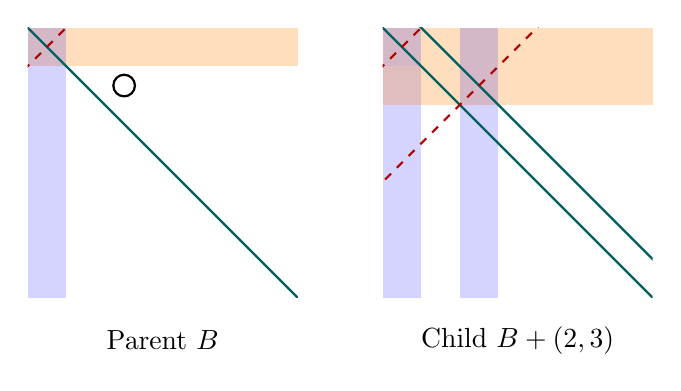
\begin{tikzpicture}[x=.49cm,y=.49cm]
 \foreach \etapa/\dx in {1/0,2/9.2}{
  \begin{scope}[shift={(\dx,0)}]
   \bcuadricula{7}
   \fill[orange,opacity=.26] (0,6) rectangle (7,7);
   \fill[blue,opacity=.17] (0,0) rectangle (1,7);
   \ifnum\etapa=2
    \fill[orange,opacity=.26] (0,5) rectangle (7,6);
    \fill[blue,opacity=.17] (2,0) rectangle (3,7);
   \fi
   \begin{scope}
    \clip (0,0) rectangle (7,7);
    \draw[teal!75!black,line width=.8pt] (.5,6.5) ++(-7,7) -- ++(14,-14);
    \draw[red!70!black,dashed,line width=.8pt] (.5,6.5) ++(-7,-7) -- ++(14,14);
    \ifnum\etapa=2
     \draw[teal!75!black,line width=.8pt] (2.5,5.5) ++(-7,7) -- ++(14,-14);
     \draw[red!70!black,dashed,line width=.8pt] (2.5,5.5) ++(-7,-7) -- ++(14,14);
    \fi
   \end{scope}
   \foreach \rr in {1,...,7}{
    \foreach \cc in {1,...,7}{
     \pgfmathtruncatemacro{\libre}{(\rr!=1)&&(\cc!=1)&&(abs(\rr-1)!=abs(\cc-1))}
     \ifnum\etapa=2
      \pgfmathtruncatemacro{\libre}{\libre&&(\rr!=2)&&(\cc!=3)&&(abs(\rr-2)!=abs(\cc-3))}
     \fi
     \ifnum\libre=1 \bmarca{7}{\rr}{\cc}\fi
    }
   }
   \breina{7}{1}{1}
   \ifnum\etapa=1
    \draw[black,line width=.8pt] (2.5,5.5) circle[radius=.28];
    \node at (3.5,-1.1) {Parent $B$};
   \else
    \breina{7}{2}{3}
    \node at (3.5,-1.1) {Child $B+(2,3)$};
   \fi
  \end{scope}
 }
\end{tikzpicture}
\caption{One transition from a parent to a child on a board of order seven. The parent has a queen
in row 1; the child is obtained by revealing row 2.
Rows are numbered from one, top to bottom, and columns from one, left to right. Crowns represent
queens already placed. The horizontal and vertical bands mark their occupied rows and columns.
Solid and dashed lines show the two families of diagonals under attack. Each dot marks an available
square. In the next row, row $2$, columns $3,4,5,6,7$ have $1,1,1,1,0$ completions, respectively,
so $Q(B)=4$. The circle marks the choice $(2,3)$ that gives the child on the right.}\label{fig:historia}
\end{figure}


\paragraph{Profile and normalization.}
Theorem~1.1 of~\cite{perfil} gives the unique optimal profile of mass one, $\nu_1$, on the unit square. We
denote its entropy by $s_1$ and write $\Phi=s_1+1$. As in~\cite{perfil,ultimas,pred}, $m_D$ and $m_A$ are
the projections of $\nu_1$ onto the two diagonal families, and $u_D=1-m_D$, $u_A=1-m_A$ are their
vacancies. For a diagonal line $f$, $m_f$ and $u_f$ denote the values at $f$ of the functions for its
family. Theorems~1.2 and~1.3 and Proposition~5.2 of~\cite{perfil} identify the positive factors and the
limit at mass one. Theorem~7.7 of the same work gives control up to the endpoint. We use the form given
in~\cite[Section~2]{pred},
\[
 \nu_1(r,c)=b_0 r_R(r)r_C(c)u_D(r-c)u_A(r+c),\qquad
 c_\nu\le\nu_1\le C_\nu,\quad \kappa_\nu\le u_D,u_A\le1.
\]
The row and column marginals of $\nu_1$ are equal to one, the factors are Lipschitz, and $L_\nu$ denotes a
Lipschitz constant for $\nu_1$, as in~\cite{pred}. The continuous coordinates of the square $(i,j)$ are
those of the center of its cell of side length $1/n$.

\paragraph{Bethe point and predictor.}
We use RC for rows and columns. As in~\cite{pred}, the \emph{Bethe point} of a residual board $B$ is the
vector $p=(p_e)$, with one weight per square in $E(B)$, at which its predictor is evaluated. It is the
stationary point of the Bethe entropy
\begin{equation}\label{bethe}
 H_B(p)=-\sum_e p_e\log p_e
       +3\sum_e(1-p_e)\log(1-p_e)-\sum_fh_f\log h_f
\end{equation}
on the domain $0<p_e<1/4$, $h_f>0$, with row and column masses equal to one. Here the \emph{mass} of a
diagonal $f$ is $\ell_f=\sum_{e\in f}p_e$, and its \emph{vacancy} is $h_f=1-\ell_f$. Physical availability
is an indicator distinct from this vacancy. On this domain $-H_B$ is strictly convex, so there is at most
one stationary point. We use the Bethe point only on the regular boards of Definition~\ref{def:regular}
and on their children, where it exists.

Suppose the row--column graph of the support is connected. Let $S_B$ be the line operator given in
Section~\ref{costes:normalizador}, and let $\pdet$ denote the product of the nonzero eigenvalues. The
predictor satisfies
\[
 L(B)=H_B(p)-\tfrac12\sum_e[\log(1-4p_e)-4\log(1-p_e)]
             -\tfrac12\log\pdet S_B+\tfrac12\log(4\pi k).
\]
The zero mode of $S_B$ is proportional to $(\mathbf1_R,-\mathbf1_C,0)$; it is the gauge of~\cite{pred}.
Deleting the row and column of $S_B$ for the same RC line gives a cofactor equal to $\pdet S_B/(2k)$,
since the corresponding component of the unit zero-mode vector has square $1/(2k)$. Thus using this
cofactor with $\tfrac12\log(2\pi)$, as in~\cite[Sections~6.1 and~7.1]{pred}, gives the same $L(B)$.

As in~\cite{pred}, the \emph{row--column Laplacian} of $p$ is the Laplacian of the graph whose vertices
are the empty rows and columns, with an edge of weight $p_e$ joining the row and column of each available
square $e$. Its \emph{gap} is its second-smallest eigenvalue. We say that $p$ satisfies a \emph{diffusion
bound} if $k\max_ep_e\le C$, that is, if no weight exceeds $C/k$; a \emph{vacancy bound} if $h_f\ge\eta$
on every diagonal; and a \emph{gap bound} if the gap is at least $\gamma$. For fixed constants
$C,\eta,\gamma>0$, these are the bounds required by Theorems~7.1 and~8.1 of~\cite{pred}. The former
assumes $k\ge\delta n$, and the latter dispenses with that condition if each diagonal has mass at most a
small $\varepsilon$.

Some notation differs from that of~\cite{pred}. There the child is written $B+c$, the row is implicit in
the ratio $\rho(B)$, which we write as $\rho(B,i)$, and the mass and vacancy of a diagonal are $m_d$ and
$h_d$. We indicate other differences as they arise. In some sections, letters such as $B$, $E$, $J$, $S$,
$T$, or $W$ denote objects defined locally. For example, in Section~\ref{permanente} the letter $B$
denotes the matrix $P-J_K$ rather than a board. Outside the abstract and introduction, $J$ does not denote
the operator of~\cite{pred}.

Some Greek letters have two uses that must not be confused. The letter $\nu$ without a subscript is
the adaptive law, whereas $\nu_1$ is always the profile and $c_\nu,C_\nu,\kappa_\nu,L_\nu$ are its
constants. The letter $\tau$ alone is the stopping time of Section~\ref{historias}, whereas $\tau_d$
and $\tau_e$, always with a subscript, are the weights of Section~\ref{costes:normalizador}. The
letter $\alpha$ alone is the constant of the introduction; the geometric threshold of
Section~\ref{meso} is written $\alpha_{\rm geo}$. In Lemma~\ref{terminal-escalado}, $\alpha$ and
$\beta$ are scaling vectors, unrelated to that constant and to the function $\beta$ of
Section~\ref{meso:constantes}.
Likewise, $F$ without arguments is the permanence event, whereas $F_{\lambda,I}$, $F_i(k)$,
$F(\sigma)$ and $F(x)$ are local objects of Sections~\ref{macro:observaciones}, \ref{meso},
\ref{costes:permanente} and~\ref{meso:regularidad}.

\paragraph{Laws for revealing and inserting queens.}
We draw a uniformly random ordering $\sigma$ of the rows. Under the \emph{uniform law} $\mu$, we choose a
uniform solution independently of $\sigma$ and reveal its queens in that order. Under the \emph{adaptive
law} $\nu$, given the next row $i$, we choose $e$ with probability
\[
 \nu_B(e\mid i)=\frac{\exp L(B+e)}{\sum_{e'\in R_i\cap E(B)}\exp L(B+e')},\qquad
 \rho(B,i)=\sum_{e'\in R_i\cap E(B)}\exp\{L(B+e')-L(B)\}.
\]
The \emph{auxiliary law} $P^{\rm B}$ uses the same uniformly chosen row and selects $e$ with
probability $p_e$. In $P^{\rm B}$ and in its expectation $\E_{\rm B}$, the upright B stands for
Bethe and does not denote a board. A \emph{history} is the resulting sequence of boards
$B_0,B_1,\dots$ together with the row order. A board with $k$ empty rows has \emph{size} $k$.
We index $B_t$ and the revealed history $\mathcal F_t$ by the number $t$ of insertions.
When indexing by size we use $B^{(k)}=B_{n-k}$ and $\mathcal F^{(k)}=\mathcal F_{n-k}$.
The latter contains the rows revealed so far and their chosen squares, before the next row is
revealed. On a stopped history these symbols refer only to levels that have been reached.
